\documentclass[a4paper, 12pt]{article}
\usepackage{graphicx}
\usepackage[numbers]{natbib}
\usepackage{amsmath}
\usepackage{parskip}
\usepackage{dsfont}
\usepackage{animate}
\usepackage{sectsty}
\usepackage[left=3cm,top=3cm,right=3cm]{geometry}

\renewcommand{\topfraction}{0.85}
\renewcommand{\textfraction}{0.1}
\allsectionsfont{\normalfont\sffamily}

\parindent=0cm

\title{Unscrambling the second law of thermodynamics}
\author{Brendon J. Brewer}

\begin{document}
\sffamily
\maketitle

The second law of thermodynamics surely qualifies as one of the most
talked-about principles in all of physics. Depending on who you ask, it is
either incredibly mysterious or fairly mundane. Some physicists think
the second law is connected to
fundamental ideas such as time and the origin of the universe
\citep{carroll}. Yet it is also an aspect of everyday experiences
such as how a morning cup of coffee cools down,
or the fact that you cannot unscramble an egg.
The second law has even been invoked by rock band {\em Muse} to
explain why, in their
view, economic growth cannot continue for much longer \citep{muse}.
Yet trying to find a clear explanation of what the second law actually is
(and why it is true) can be a frustrating experience.

I first encountered the second law
as a teenager, while reading an issue of the fundamentalist Christian magazine
{\em Creation} given to me by my grandmother. Since the magazine wanted to
argue against biological evolution, it claimed that the second law of
thermodynamics implies evolution is impossible. Its definition of the second
law was that {\em disorder always increases with time}.
At first glance, this does seem incompatible with evolution by
natural selection, which can lead to more complex,
``better designed'' organisms over time \citep{dawkins}.
At the time, I thought it was unlikely that mainstream biology would flagrantly
contradict mainstream physics, so I remained sceptical of this argument,
even though I couldn't understand the counterarguments I found on the
internet at the time.

During my first university physics course, I was excited when I learned
we'd be
studying thermodynamics. Finally, I thought, I would be able to understand the
second law properly (along with the other, less popular laws).
Alas, my expectations were not met, despite having a good lecturer.
Instead of discussing big picture issues like evolution, economics, or
cosmology, we
worked out the maximum possible efficiency of refrigerators and steam engines
I'm sure these are interesting in their own ways, but I was disappointed.
The version of the second law we studied was related to concepts of heat
and temperature, and little else.
A familiar consequence of this version of the second law is that
heat always flows from a hot object to a cooler
one, and not the other way around. Your morning
cup of coffee cools down, and heats up the air around it: it doesn't heat
up further while cooling the room, even though that possibility is compatible
with other laws of physics such as the conservation of energy.

The second law is formalised by defining a quantity called
{\em entropy}. When heat flows {\em out of} one object and into another,
the first object's entropy goes
down, by an amount that depends on its temperature.
The change in the entropy is the amount of heat energy transferred,
$Q$ (usually measured in joules)
divided by the temperature of the object, $T_1$, measured in Kelvin.
When that same heat energy flows {\em into} another object, that object's
entropy goes up by $Q$ divided by the temperature of the
second object, $T_2$. The second law of thermodynamics can then be stated: if you
add up all of the changes in entropy of all the objects you are studying,
the result must be a positive number or zero. It can't be negative. In other
words, the total entropy must either increase or stay the same.
When a cup of coffee cools down its entropy decreases, but the entropy of its
surroundings increases by an even greater amount,
since the coffee is hotter than the surroundings.

The version of
the second law I just described, usually attributed to the 19th century
German physicist Rudolf Clausius, certainly has its uses. However it is a far
cry from the lofty fundamental principle I had expected to learn. What did it
have to do with evolution? The fact that organisms seem designed doesn't have
anything to do with heat being transferred. And it doesn't have much to do
with the economy either, except very indirectly because machines are useful
and the second law says some kinds of machines aren't possible.

Confusingly, as we learned the Clausius version of the second law, we also
discussed phenomena such as gas diffusion, shown in this animated gif:

%Animated gif in the public domain, obtained from:
%https://commons.wikimedia.org/wiki/File:Diffusion_animation.gif
\begin{figure}[ht!]
\centering
\animategraphics[scale=0.5]{12}{frame-}{0}{108}
\end{figure}

In the animation, purple gas atoms start above the horizontal barrier in the
middle of the box, and green atoms start below the barrier.
As time progresses, the purple and green atoms end up spread throughout the entire
box. This ``spreading out'', in a physical sense, was claimed to be an example
of the second law. Yet I could never find what heat was being transferred
in this example. If no heat is being transferred, the Clausius second law
doesn't apply --- we are left with hand waving about disorder.

So {\em is there} a version of the second law that relates to concepts more
general than heat and temperature?
It turns out the answer is yes, but I had to wait many years before I learned it.
Surprisingly, it turns out this more general second law isn't really a
principle of {\em physics}, but rather a
principle of {\em reasoning}. And this more general version of the
second law not only explains why the Clausius version is true, but gives us
a tool for much more general questions --- like the evolution question.
It also appears in everyday life, and not just in situations involving heat and
temperature. For example,
why is darts difficult? Why can't most men sing operatic high Cs?
And why are political polls (somewhat) accurate?

\section*{Uncertainty and volume}
During my PhD studies, I became intensely interested in Bayesian statistics
\citep{brewer}
and how to use it in astronomical data analysis. During this process I
discovered the work of the heterodox physicist E. T. Jaynes \citep{jaynes_site}
(1922--1988), whose clear-headed thinking and combative writing style
changed the direction of my PhD project and my life.

One day I came across a particular Jaynes paper, which is now one of my
favourite journal articles of all time
\citep{jaynes}. I didn't understand it
immediately, but had a strong sense that I should persist because it seemed
important. Every so often, I'd return to re-read it, understanding
just a little more each time. The breakthrough came after dinner one
night.

I had taken out a tub of ice cream from the freezer for dessert. After dishing
the ice-cream into a bowl, I tried putting the tub back in the freezer, but
it wouldn't fit. Suddenly it clicked: Jaynes was explaining that
the second law of thermodynamics, both the Clausius heat/temperature version
and (importantly) a more general version, reduce to the
principle that {\em big things cannot fit into small spaces unless they are
compressed}. This is common sense when applied to physical objects, but to
get the second law, you have to apply it to an abstract object: a volume
of possibilities. This idea did not necessarily originate with Jaynes, as it
can be found (albeit less explicitly stated)
in the work of chemist J. Willard Gibbs, among others. Another source that
helped me understand it was the posts of irreverant blogger ``Pierre Laplace''
\citep{pierre_laplace}.

To demonstrate the idea of a volume of possibilities,
consider the 52 books on my office bookshelf\footnote{This
is actually true, and it's a coincidence that there are 52 cards in a standard
deck of cards. I try to avoid explanations involving cards, coin flipping, and
dice, because people think they understand those already.}.
Only two of the books on the shelf are fiction, since I prefer to read
non-fiction, and it also makes more sense to have non-fiction books in an
office. Now I tell you that one of the books on the shelf was
signed by the author. Which one? I'm not telling. Based solely on this
information, it makes sense for you to assign a probability of 1/52 to each of the
books, describing how plausible you think it is for each book to be the signed
one.

From this state of near-ignorance, it seems like you might not be able to draw
any conclusions with a high confidence. But that's an illusion: it depends on
what questions you ask. Imagine if I were to ask you whether the signed book
is a non-fiction book. If your probability is 1/52 for each book being the
signed one, the probability the signed one is non-fiction must be
50/52 (adding the probabilities of the 50 non-fiction books together), 
or approximately 96\%. That's an impressive level of confidence --- much more than you should have in the conclusion of a single peer-reviewed science paper!
Of course, a high probability doesn't mean the result (the signed book is
non-fiction) is guaranteed. It just means it's very plausible {\em based on the
information that you explicitly put into the calculation}.

Here is a (very simple) diagram of my bookshelf, with the blue regions
being non-fiction books, and the red being fiction:
\begin{figure}[ht!]
\centering
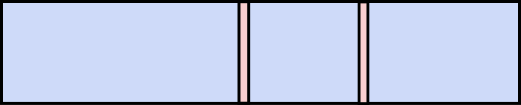
\includegraphics{bookshelf.png}
\end{figure}
Clearly the safest bet is that the signed book is non-fiction, simply because
there are more of them --- they occupy a large majority of the volume of
possibilities (which, in this case, corresponds to a physical volume on my
bookshelf). A safe bet is, however, not a guarantee.

The general principle here, which Jaynes pointed out, is this:
{\em If you consider all possibilities that are consistent with
the information you have, and the vast majority of those possibilities
imply a certain outcome that is meaningful to you, then that outcome is very
plausible}. This is also a consequence of probability theory. The only
way around this conclusion is to have some reason to assign highly
non-uniform probabilities to the possibilities --- for example, if I had
some reason to assign high probabilities to the two fiction books.

%Now, what happens if I rearrange the books in an arbitrary manner? All the books
%will be in a different order, and in terms of fiction vs. non-fiction, the
%latter will still dominate:
%\begin{figure}[ht!]
%\centering
%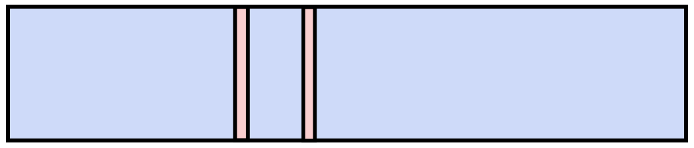
\includegraphics[scale=0.61]{bookshelf2.png}
%\end{figure}
%After this, there's still a 96\% probability the signed book is non-fiction.

\section*{Clausius from Jaynes}
%Discuss the Clausius second law as a consequence of the Jaynes one
The Gibbs/Jaynes version of the second law can be applied to all sorts of
questions, and it can also explain why the Clausius version, about heat and
temperature, is true. 

When I say that I have a hot cup of coffee and that the air around it is cooler,
it seems like quite a specific statement. But in a certain sense it is actually
a very vague statement, in that it leaves out a large number of details about
what's actually happening. I didn't tell you the colour of the mug, whether
my window was open, whether the coffee was instant or not (usually instant with
soy milk and two pills of sucralose if you're wondering...I can handle the hate mail). More conventionally, it also left out a huge number of details about the position and
velocity (speed and direction of movement) of every molecule in the mug and
the surrounding air. The the high temperature of the coffee means its
molecules are moving fairly rapidly, but there's precious little information
apart from that.

Based on this very vague information about the cup of coffee, can we predict
what will happen in the future? Our common sense and experience say yes, very
loudly. Hot cups of coffee cool down. Duh!
But to a physicist the standard way of predicting the future is to use
the laws of motion, which predict how particles (such as molecules of coffee
and air) will move around. The catch is that we need to give the {\it initial
conditions}: what are all the positions and velocities that we're making our
prediction {\it from}?

Since we don't know the initial conditions (we only have the `vague' information
about the temperature) we can't actually apply the standard laws of motion to
see what will happen in the future. Any prediction we make will be a
guess, or more formally, a probability. We're in a situation analogous to the
bookshelf one. 

If we think of all possibilities for what the positions and velocities of the
coffee and air molecules might be, the vague information we have
can only restrict the possibilities down to a subset, shown as the red area
below:

\begin{figure}[ht!]
\centering
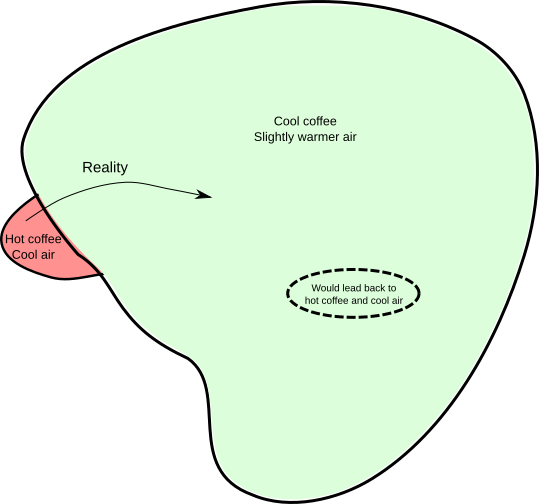
\includegraphics[scale=0.6]{diagrams.png}
\end{figure}

Now, what the laws of motion will do for you is tell you how a point in this
diagram will move around over time
(equivalently, how the positions and velocities of all the molecules will
move over time). For an actual situation, at a particular instant, the physical
reality is represented by a single point somewhere in the red zone. As time
goes on, that point will move around (as depicted by the curved arrow in
the diagram). Where will it end up? That depends on precisely where in the
red zone the point was initially.

However, notice that the red zone is much smaller than the 



I must admit that when I hear `entropy' from a physicist without a long
set of qualifications, I don't know what they're talking about. Most will
happily talk about ``the entropy of the universe'' being low in the past,
or how Stephen Hawking derived the ``entropy of a black hole''.
I don't know what these statements mean,
and I don't think it's entirely my fault.
There seems to be little recognition of the fact
that the {\em exact same physical system}
can have more than one entropy, depending on how we want to think about it.
Entropy describes what is known about a system, or how much information a
vague statement provides about the system. There is no `true' entropy that
we could calculate {\bf even if we knew everything that there was to be known!}
What {\em rules of thumb} are we looking for? Different ones may exist, and
we'll find them by using different entropies.

Interestingly, this explanation doesn't really explain anything about time,
since notions of time were assumed in the explanation itself. Presumably,
a more fundamental explanation for time would explain it in terms of some
other concepts.

\section*{Entropy is about what is known, not what is there}
%{\textsf \textbf Write about how the same physical system can have different entropies}

It's worth thinking about whether the second law really does forbid evolution
by natural selection. We don't need to get particularly technical with the
concept of entropy in order to have a go at that. All we need to ask is whether
it's plausible that a population of self-replicating organisms will tend to
`improve' their survival and reproductive `fitness' over time.
The answer is yes, provided the mutation rate is sufficiently
low. And if the organisms reproduce sexually, the population's average fitness
will increase even faster \citep{mackay}. This isn't the Clausius version of
the second law, but an example of the Jaynes one: of all the possible deaths,
reproduction events, and mutations that could plausibly occur, most would lead to
an increase in the average fitness of the population.

\section*{The second law in ordinary life}
As promised, the more general second law can be applied to everyday questions.
One of my favourite analogies is singing. About ten years ago, I decided to
learn how to sing, since it seemed fun, and not having to carry an instrument
around has its advantages. Back then I couldn't sing very well and in particular
I couldn't sing above E4, the E just above middle C. This was frustrating but
very common: the male singers you hear on the radio tend to sing songs with
notes well above that, apparently with ease. Why couldn't I?

It turns out that singing high notes requires very specific conditions to be
achieved in the larynx, regarding air pressure and so on. To get this right,
you need to apply muscular effort in your torso in a particular way that singers
traditionally call support \citep{cvt}. You also can't be quiet unless you want
a very gentle ``falsetto'' sound. The volume required is more than most people
would intuitively feel is necessary. For example, I can't sing high-pitched
rock songs while my wife is in the same room because it hurts her ears.


\begin{thebibliography}{999} % if there are less than 10 entries, enter a one digit number
\bibitem[]{carroll}
Carroll, Sean. From eternity to here: the quest for the ultimate theory of time. Penguin, 2010.

\bibitem[]{muse}
Muse. The 2nd law.
http://www.allmusic.com/album/the-2nd-law-mw0002406726

\bibitem[]{dawkins}
Dawkins, Richard. The blind watchmaker: Why the evidence of evolution reveals a universe without design. WW Norton \& Company, 1986.

\bibitem[]{brewer} The Great Statistical Schism. Quillette, 2015.
http://quillette.com/2015/11/13/the-great-statistical-schism/

\bibitem[]{jaynes_site}
http://bayes.wustl.edu/

\bibitem[]{jaynes}
Jaynes, Edwin T.
Gibbs vs Boltzmann entropies. American Journal of Physics 33.5 (1965): 391-398.

\bibitem[]{pierre_laplace}
http://www.bayesianphilosophy.com/

\bibitem[]{cvt}
Sadolin, Cathrine, Complete Vocal Technique, Copenhagen 2012.
ISBN 978-87-992436-7-9.

\bibitem[]{mackay}
David MacKay, Information Theory, Inference, and Learning Algorithms.
Chapter 19.
http://www.inference.phy.cam.ac.uk/mackay/itprnn/ps/265.280.pdf

\end{thebibliography}

\end{document}

